%%%%%%%%%%%%%%%%%%%%%%%%%%%%%%%%%%%%%%%%%%%%%%%%%%%%%%%%%%%%%%%%%%%%%%%%%%%%%%%%%%
%%      Template using LaTeX  Tutorial tex files								%%
%%      																		%%
%%      Copyright Rho Vector Latex Tutorial 2021								%%
%%		rhovector <rhovector@gmail.com>			 								%%
%%		vivekadi <vivek.adishesha@gmail.com>,									%%
%%		chiranjitpatel <chiranjitpatel08@gmail.com>								%%
%%																				%%
%%																				%%	
%%      This program is FREE SOFTWARE; you can redistribute it and/or modify	%%
%%      it under the terms of the GNU General Public License as published by	%%
%%      the Free Software Foundation; either version 2 of the License, or		%%
%%      (at your option) any later version.										%%
%%      																		%%
%%      This program is distributed in the hope that it will be useful,			%%
%%      but WITHOUT ANY WARRANTY; without even the implied warranty of			%%
%%      MERCHANTABILITY or FITNESS FOR A PARTICULAR PURPOSE.					%%
%%      See GNU General Public License for more details.						%%
%%      																		%%
%%      You should have received a copy of the GNU General Public License		%%
%%      along with this program; if not, write to the Free Software				%%
%%      Foundation, Inc., 51 Franklin Street, Fifth Floor, Boston,				%%
%%      MA 02110-1301, USA.														%%
%%%%%%%%%%%%%%%%%%%%%%%%%%%%%%%%%%%%%%%%%%%%%%%%%%%%%%%%%%%%%%%%%%%%%%%%%%%%%%%%%%


\documentclass{memoir}
\usepackage[utf8]{inputenc}
\usepackage[english]{babel}

\usepackage{chemfig}
\usepackage{modiagram}

\usepackage{graphicx}
\usepackage{geometry}
\usepackage{float}
\usepackage{subcaption}
\usepackage{caption}


\usepackage{pgfplots}
\pgfplotsset{width=10cm,compat=1.9}



\begin{document}

\chapter{Latex Introduction \& Applications}

\section{History \& Introduction}
\begin{itemize}
	\item \textbf{LaTeX is a software system for document preparation.}
	\item \textit{Created in the early 1980s by Leslie Lamport.}
	\item \textit{LaTeX 2e, the current standard version.}
	\item \textbf{Free software.} 
\end{itemize}

\section{Images}

\begin{figure}[H]
	\centering
	\begin{subfigure}{0.5\linewidth}
		\centering
		\includegraphics[width=0.5\linewidth]{"newton"}
		\caption{Issac Newton}
		\label{fig:mg995_1}
	\end{subfigure}%
	\begin{subfigure}{0.5\linewidth}
		\centering
		\includegraphics[width=0.5\linewidth]{"tesla"}
		\caption{Nikola Tesla}
		\label{fig:mg995-schematic}
	\end{subfigure}
	\caption{Famous scientists}
	\label{fig:mg995_schema}
\end{figure}

\section{Drawing shapes}

\begin{tikzpicture}
	
	\draw[blue, very thick] (0,0) rectangle (3,2);
	\draw[orange, ultra thick] (4,0) -- (6,0) -- (5.7,2) -- cycle;
	
\end{tikzpicture}

\section{Tables}

\begin{table}[H]
	\centering
	\caption{Coefficients of Exponential fit -> Box-3 for Z-Coordinate map}
	\begin{tabular}{cc}
		\hline 
		Parameter & Value (95\% Confidence) \\ 
		\hline 
		a & 41.28 (36.01, 46.55) \\  
		b & -0.1734 (-0.1965, -0.1502) \\ 
		c & 29.08 (27.79, 30.36) \\  
		d & -0.01035 (-0.01152, -0.009181) \\  
		SSE & 1.49 \\ 
		R-square & 0.9987 \\  
		RMSE & 0.2096 \\ 
		\hline 
	\end{tabular}
	\label{tab:box3-coeff}
\end{table}

\section{Chemical Graphs}
Double bond
\chemfig{O=H}
\\
Regular polygons
\chemfig{A*5(-B=C-D-E=)}
\\
Incomplete rings are also possible
\chemfig{A*5(-B=C-D)}
\\
Branched molecule \vspace{.5cm}
\chemfig{H-C(-[2]H)(-[6]H)-C(=[1]O)-[7]H}


\section{Molecular Orbitals}
\begin{modiagram}
	\atom{left}{
		1s, 2s, 2p = {;pair,up,up}
	}
	\atom{right}{
		1s, 2s, 2p = {;pair,up,up}
	}
	\molecule{
		1sMO, 2sMO, 2pMO = {;pair,pair,pair,up,up}
	}
\end{modiagram}


\section{Plotting Graphs}

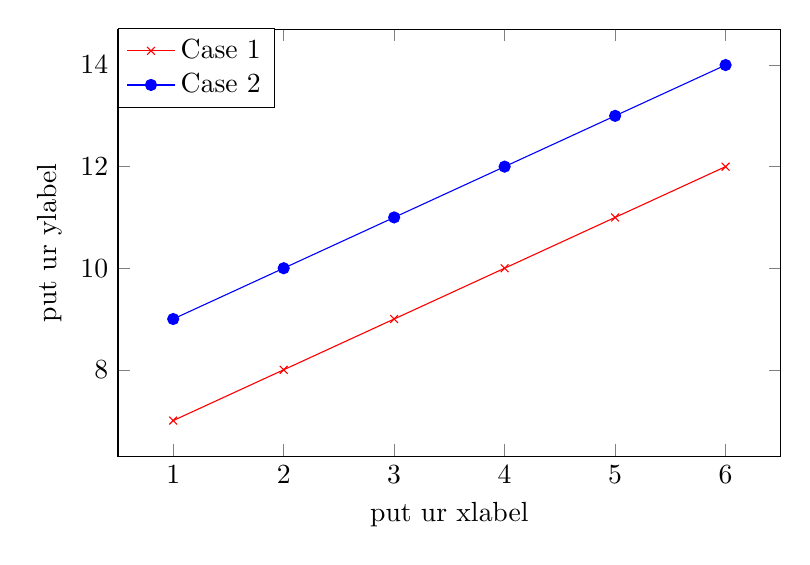
\begin{tikzpicture}
	\begin{axis}[
		xlabel=put ur xlabel,
		ylabel=put ur ylabel,
		width=10cm,height=7cm,
		legend style={at={(0.0,.91)},anchor=west}]
		\addplot[color=red,mark=x] coordinates {
			(1, 7)
			(2, 8)
			(3, 9)
			(4, 10)
			(5, 11)
			(6, 12)
		};
		
		\addplot[color=blue,mark=*] coordinates {
			(1, 9)
			(2, 10)
			(3, 11)
			(4, 12)
			(5, 13)
			(6, 14)
		};
\legend{Case 1,Case 2}
\end{axis}
\end{tikzpicture}

	
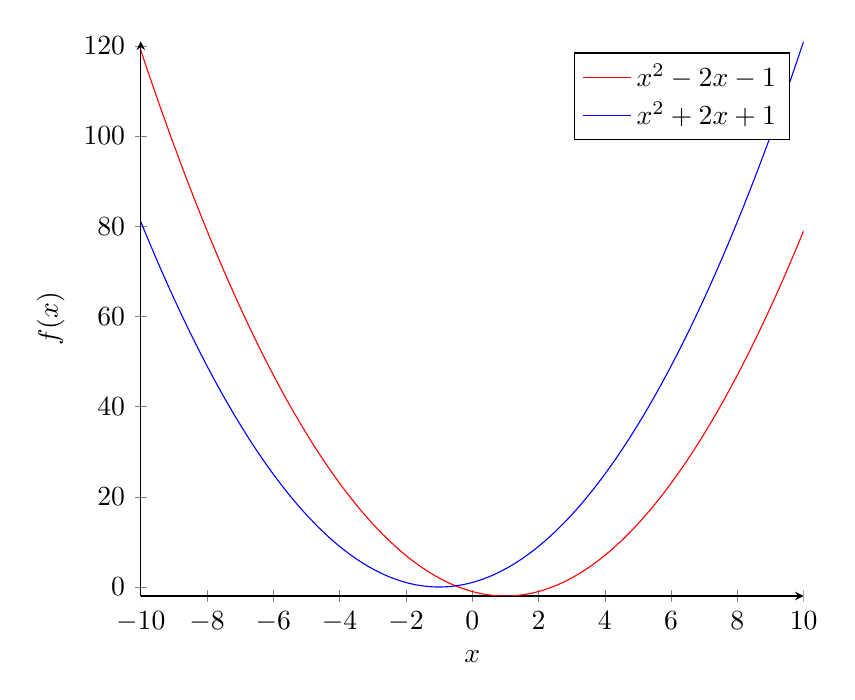
\begin{tikzpicture}
	\begin{axis}[
		axis lines = left,
		xlabel = \(x\),
		ylabel = {\(f(x)\)},
		]
		%Below the red parabola is defined
		\addplot [
		domain=-10:10, 
		samples=100, 
		color=red,
		]
		{x^2 - 2*x - 1};
		\addlegendentry{\(x^2 - 2x - 1\)}
		%Here the blue parabola is defined
		\addplot [
		domain=-10:10, 
		samples=100, 
		color=blue,
		]
		{x^2 + 2*x + 1};
		\addlegendentry{\(x^2 + 2x + 1\)}
		
	\end{axis}
\end{tikzpicture}


\section{Math Equations}
	\[    \alpha^2 + \beta^2 = \gamma^2      \]
	
	\[		\log(xy) = \log x	+ \log y							\]
	
	\[		F = G \frac{m_1m_2}{r^2}								\]
	
	
	\[		\phi(x) = \frac{1}{\sqrt {2\pi\sigma}}		e^{-\frac{(x-\mu)^2}	{2\sigma^2}	}										\]
	
	
	\[		\frac{{\partial ^2}u}   {\partial {t^2}}	= {c^2}	 		\frac{{\partial ^2}u}   {\partial {x^2}}		\]
	
	
	\[		f(w) = \int\limits_{- \infty} ^{\infty}		f(x) e^ {-2\pi ixw}	dx				\]
	
	\[		\nabla \cdot E = \frac {\rho} {\varepsilon _0}			\]


\end{document}
